\section{Nutmeg \& Mace}
\label{sec:nutmeg}
\label{sec:mace}

\begin{spice}\label{spice:nutmeg}
\textsc{Nutmeg} \hfill \href{https://powo.science.kew.org/taxon/586076-1}{POWO} \\
\textbf{English:} \textit{nutmeg}. 
\textbf{Arabic:} {\arabicfont{جوز الطيب}} \textit{jawz al-ṭīb} [fragrant nut]; nan. 
\textbf{Chinese:} {\tradchinesefont{肉豆蔻}} \textit{ròudòukòu} [flesh-bean-cardamom]. 
\textbf{Hungarian:} \textit{szerecsendió} [Saracen nut]; \textit{muskátdió} [musk-nut]; \textit{mácisdió} [mace-nut].  \\
\noindent{\color{black}\rule[0.5ex]{\linewidth}{.5pt}}
\begin{tabular}{@{}p{0.25\linewidth}@{}p{0.75\linewidth}@{}}
Plant species: & \taxonn{Myristica fragrans}{Houtt.} \\
Family: & \textit{Myristicaceae} \\
Plant part used: & seed \\
Region of origin: & Moluccas (Indonesia) \\
Cultivated in: & Grenada, Indonesia \\
Color: & pale brown nut, dark when powdered \\
\end{tabular}
\end{spice}

\begin{figure}[!ht]
	\vspace{-4ex}
	\centering
	\subfloat[\centering a]{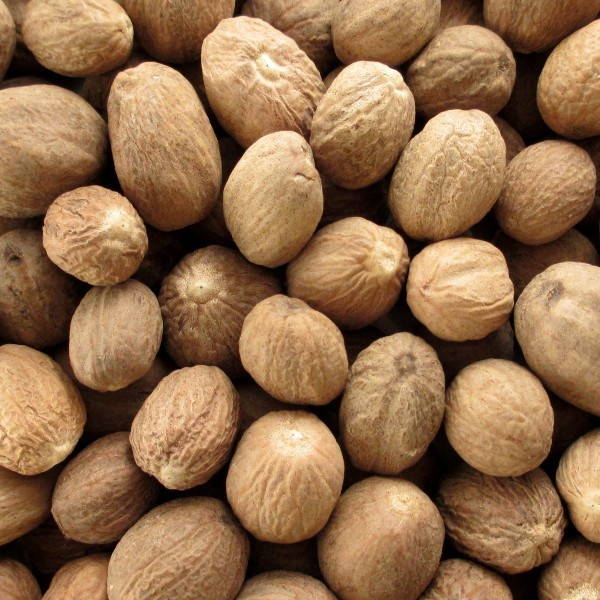
\includegraphics[width=0.3\linewidth]{imgs/spices/nutmeg-2.jpg}}
	\hfill
	\subfloat[\centering b]{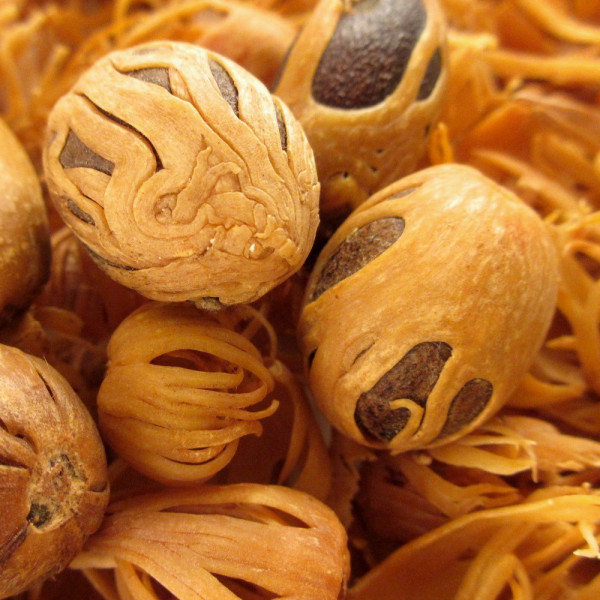
\includegraphics[width=0.3\linewidth]{imgs/spices/mace-1.jpg}}
	\hfill
	\subfloat[\centering c]{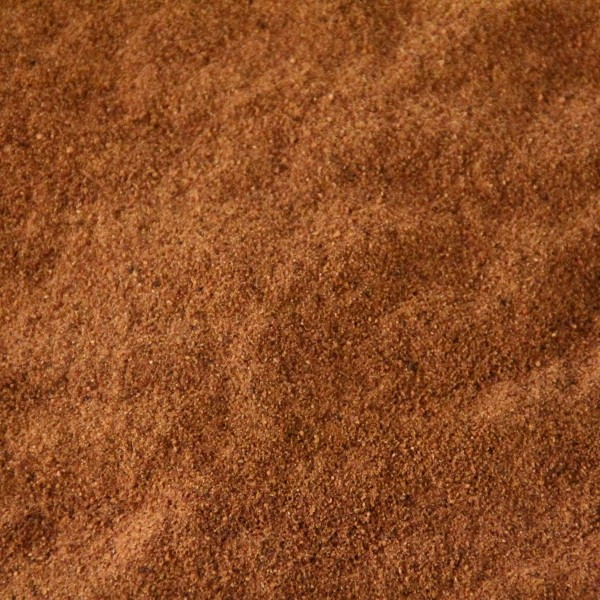
\includegraphics[width=0.3\linewidth]{imgs/spices/nutmeg-3.jpg}}
	\caption{Nutmeg, \taxon{Elettaria nutmegum}.}
	\label{fig:nutmeg_imgs}
\end{figure}

\begin{spice}\label{spice:mace}
\textsc{Mace} \hfill \href{https://powo.science.kew.org/taxon/586076-1}{POWO} \\
\textbf{English:} \textit{mace}. 
\textbf{Arabic:} {\arabicfont{بسباسة}} \textit{basbāsa}; {قشرة جوز الطيب} \textit{qishrat jawz al-ṭīb} [the peel of the fragrant nut]. 
\textbf{Chinese:} {\traditionalchinesefont{肉豆蔻皮}} \textit{ròudòukòupí} [flesh-bean-cardamom-skin]. 
\textbf{Hungarian:} \textit{szerecsendió-virág} [Saracen nut flower].  \\
\noindent{\color{black}\rule[0.5ex]{\linewidth}{.5pt}}
\begin{tabular}{@{}p{0.25\linewidth}@{}p{0.75\linewidth}@{}}
Plant species: & \taxonn{Myristica fragrans}{Houtt.} \\
Family: & \textit{Myristicaceae} \\
part used: & aril \\
Region of origin: & Moluccas (Indonesia) \\
Cultivated in: & Grenada; Indonesia \\
Color: & crimson red aril whn fresh, pale yellow when dried \\
\end{tabular}
\end{spice}

% \begin{figure}[!ht]
% 	\vspace{-4ex}
% 	\centering
% 	\subfloat[\centering a]{\includegraphics[width=0.3\linewidth]{imgs/spices/mace1.jpg}}
% 	\hfill
% 	\subfloat[\centering b]{\includegraphics[width=0.3\linewidth]{imgs/spices/mace2.jpg}}
% % 	\hfill
% % 	\subfloat[\centering c]{\includegraphics[width=0.3\linewidth]{imgs/spices/mace3.jpg}}
% 	\caption{Mace, \taxon{M}.}
% 	\label{fig:mace_imgs}
% \end{figure}

\subsection{The Botany of Nutmeg}

\subsection{The History of Nutmeg}

\subsection{The Names of Nutmeg}

\subsubsection{English}

\begin{etymology}\label{ety:nutmeg}
English \textit{nutmeg}
< Anglo-Norman \textit{*nois mugue}
< Old French \textit{nois mug(u)ede; nois musguete}
< Romance* \textit{*nuce muscāta}
< Latin \textit{nux muscada}
< Pahlavi \textit{*mušk}
< Sanskrit \textit{muṣka}\footnote{; }
\end{etymology}

\begin{table}[!ht]
\centering
\begin{tabularx}{\textwidth}{@{}l>{\itshape \small}lL>{\small}l@{}}
\toprule
\textbf{\#} & \multicolumn{1}{l}{\textbf{Species}} & \multicolumn{1}{l}{\textbf{Name}} & \multicolumn{1}{l}{\textbf{Source}} \\
\midrule
\textbf{1}	& \textbf{Myristica fragrans}	& \textbf{nutmeg}	& \textbf{\textcite{van_wyk_culinary_2014}} \\
\bottomrule
\end{tabularx}
\caption{Various names for nutmeg in English.}
\label{table:names_nutmeg_en}
\end{table}



\subsubsection{Arabic}

\begin{table}[!ht]
\centering
\begin{tabularx}{\textwidth}{@{}l>{\itshape \small}lr>{\itshape}lL>{\small}l@{}}
\toprule
\textbf{\#} & \multicolumn{1}{l}{\textbf{Species}} & \multicolumn{1}{l}{\textbf{Name}} & \multicolumn{1}{l}{\textbf{Tr.}} & \multicolumn{1}{l}{\textbf{Gloss}} & \multicolumn{1}{l}{\textbf{Source}} \\
\midrule
1	& Myristica fragrans	& داركيسة	& dārkīsa	& 	& \textcite{amar_arabian_2017} \\
\textbf{2}	& \textbf{Myristica fragrans}	& \textbf{جوز الطيب}	& \textbf{jawz al-ṭīb}	& \textbf{fragrant nut}	& \textbf{\textcite{amar_arabian_2017}} \\
3	& Myristica fragrans	& جوز بوى	& jawz bawwā	& fragrant nut	& \textcite{amar_arabian_2017} \\
\bottomrule
\end{tabularx}
\caption{Various names for nutmeg in Arabic.}
\label{table:names_nutmeg_ar}
\end{table}



\subsubsection{Chinese}

\begin{table}[!ht]
\centering
\begin{tabularx}{\textwidth}{@{}l>{\itshape \small}ll>{\itshape}lL>{\small}l@{}}
\toprule
\textbf{\#} & \multicolumn{1}{l}{\textbf{Species}} & \multicolumn{1}{l}{\textbf{Name}} & \multicolumn{1}{l}{\textbf{Tr.}} & \multicolumn{1}{l}{\textbf{Gloss}} & \multicolumn{1}{l}{\textbf{Source}} \\
\midrule
\textbf{1}	& \textbf{Myristica fragrans}	& \textbf{\traditionalchinesefont{肉豆蔻}}	& \textbf{ròudòukòu}	& \textbf{flesh-bean-cardamom}	& \textbf{\textcite{defrancis_abc_2003}} \\
2	& Myristica fragrans	& \traditionalchinesefont{肉荳蔻籽粉}	& ròudòukòuzǐfěn	& flesh-bean-cardamom-seed-powder	& \textcite{kleeman_oxford_2010} \\
\bottomrule
\end{tabularx}
\caption{Various names for nutmeg in Chinese.}
\label{table:names_nutmeg_zh}
\end{table}



\subsubsection{Summary}

\begin{table}[!ht]
\centering
\begin{tabularx}{\textwidth}{@{}ll>{\itshape}lLl>{\small}l@{}}
\toprule
\textbf{\#} & \textbf{Language} & \multicolumn{1}{l}{\textbf{Term}} & \textbf{Gloss} & \textbf{Loan} & \multicolumn{1}{l}{\textbf{Source}} \\
\midrule
1	& English	& nutmeg	& 	& yes	& \textcite{oed} \\
\midrule
1	& Arabic	& jawz al-ṭīb	& fragrant nut	& yes	& \textcite{wehr_dictionary_1976} \\
2	& Arabic	& jawz bawwā	& fragrant nut	& yes	& \textcite{baalbaki_-mawrid_1995} \\
\midrule
1	& Chinese	& ròudòukòu	& flesh-bean-cardamom	& no	& \textcite{defrancis_abc_2003} \\
2	& Chinese	& ròudòukòuzǐfěn	& flesh-bean-cardamom-seed-powder	& no	& \textcite{kleeman_oxford_2010} \\
\bottomrule
\end{tabularx}
\caption{Conventionalized names for nutmeg in English, Arabic, and Chinese, found in dictionaries.}
\label{table:names_nutmeg}
\end{table}
















% Moreover, remnants of nutmeg were found at al-Dayr al-Baªrī (sixteenth to fourteenth centuries BC).111
% Amar 



















% English,nutmeg
% Middle English,notmyg; nutemug(g)e
% Anglo-Norman,*nois mugue
% Old French,nois mug(u)ede; nois musguete
% Romance,*nuce muscāta
% Latin,nux muscada
% Pahlavi,*mušk
% Sanskrit,muṣka

% EE:
% XIV. ME. nute-, notemug(g)e, later notmyg (XV), note-, nutmeg (XVI), partial tr. of AN. *nois mugue, for OF. nois mug(u)ede (also musguete; now noix muscade) :- Rom *nuce muscāta ‘musk-smelling nut’ (L. nux NUT, muscus MUSK).

% OE:
% "hard aromatic seed of the fruit of a tree found in the East Indies," used as a spice on cookery, c. 1300, note-mug, from Old North French or Anglo-French *noiz mugue, from Old French nois muguete, an unexplained alteration of nois muscade "nut smelling like musk," from nois "nut" (from Latin nux, from PIE *kneu- "nut;" see nucleus) + Latin muscada, fem. of muscat "musky" (see muscat). Probably influenced in English by Medieval Latin nux maga (compare unaltered Dutch muskaatnoot, German muscatnuß, Swedish muskotnöt).

% American English colloquial wooden nutmeg "anything false or fraudulent" is from 1827; Connecticut is called the Nutmeg State "in allusion to the story that wooden nutmegs are there manufactured for exportation." [John Russell Bartlett, "Dictionary of Americanisms," 1859]

%     At a dinner party, the other day, during a little playful discussion of Yankee character, a bland and benevolent-looking old gentleman at my side informed me that he had come to the conclusion that the wooden-nutmeg story was neither more nor less than a mischievous satire. "For," said he, "there would be such an amount of minute carving required to make a successful imitation of the nutmeg, that the deception would hardly pay the workman. For myself, I do not believe the cheat was ever practised." I thanked him in the name of my country for the justice done her, and assured him that the story of the Yankee having whittled a large lot of unsaleable shoe-pegs into melon seeds, and sold them to the Canadians, was also a base fabrication of our enemies. [Grace Greenwood, "Haps and Mishaps of a Tour in Europe in 1853"]

% MW:
%Middle English notemuge, partial translation, partial modification of Old French nois muguete, nois muguede nutmeg, alteration of nois muscade, from Old Provençal noz muscada, from noz nut (from Latin nuc-, nux) + muscada, feminine of muscat musky — more at nut, muscat
%First Known Use: 15th century (sense 1a)

% AH:
% [Middle English notemuge, probably ultimately from Old French nois mugede, alteration of nois muscade, nut smelling like musk, from Old Provençal notz muscada : notz, nut (from Latin nux, nuc-, nut) + muscada, smelling like musk (from musc, musk, from Late Latin muscus; see MUSK). N., sense 4 and v., perhaps from earlier slang nutmegs, testicles, or current slang nuts, testicles (since the nutmegged ball passes between the defender's legs) or perhaps from rhyming slang nutmeg, leg.]

% WK:
% From Middle English notemege, notemuge, a partial translation of Medieval Latin nux muga, a variant of Medieval Latin nux muscata (“musky nut”). Compare also Old French nois mugede. 



\begin{spice}
\textit{Myristica fragrans} Houtt. \hfill \href{https://powo.science.kew.org/taxon/586076-1}{POWO}\\
\textbf{English}: \textit{mace}.
\textbf{Chinese}: 肉荳蔻皮 \textit{ròudòukòupí}.
\textbf{Arabic}: قشرة جوز الطيب \textit{qišratu jawzi ṭ-ṭībi}, بسباس \textit{basbās}.
\textbf{Hungarian}: \textit{szerecsendió-virág}.
\end{spice}

\begin{etymology}
English \textit{mace} XIV (back-formation, false sg. from percieved pl. \textit{macis}) EE XIII MW
< Middle English \textit{macis, maces, mace} MW
< Middle French \textit{maci; macis} AH
< Medieval Latin \textit{macis} misreading? AH
< Old French \textit{macis} EE OE
< Latin \textit{macir} `red spicy bark from India' EE OE `reddish rind of an Indian root' MW `red bark of the root of a South Asian tree (possibly Holarrhena antidysenterica) used as a remedy for dysentery' AH
< Ancient Greek \textit{mákir} MW AH
< unknown, Oriental loanword 
\end{etymology}



% EE:
% outer covering of the nutmeg. XIV (macis). — AL. or (O)F. macis — L. macir red spicy bark from India; the form macis being apprehended as a pl., a new sg. mace was formed from it.

%OE:
%mace (n.2)
%"spice made from dry outer husk of nutmeg," late 14c., from Old French macis (in English taken as a plural and stripped of its -s), a word of uncertain origin, sometimes said to be a scribal error for Latin macir, the name of a red spicy bark from India, but OED finds this etymology unlikely.

%MW
%% Middle English mace, macis, from Middle French maci, macis, from Latin macir reddish rind of an Indian root, from Greek makir, makeir
% First Known Use: 13th century (sense 1)

%AH
% [Middle English, back-formation from macis, maces, mace (taken as a plural ending in -s), ultimately (partly via Old French macis) from Medieval Latin macis, perhaps from misreading of Latin macir, the red bark of the root of a South Asian tree (possibly Holarrhena antidysenterica) used as a remedy for dysentery, from Greek makir, of unknown origin.]




Why is Connecticut called 'The Nutmeg State'?
https://www.ctpost.com/living/article/Why-is-Connecticut-called-The-Nutmeg-State-16233291.php